\chapter{Smart Card}

La Smart Card è, a tutti gli effetti, un microcomputer dotato di un proprio sistema operativo, seppur in una versione semplificata. Questo tipo di dispositivi nasce principalmente per garantire la protezione dei dati (come nel caso dei bancomat) o per memorizzare in modo sicuro password e chiavi crittografiche, come abbiamo visto precedentemente con Kerberos. Le loro applicazioni sono vastissime e spaziano dalla classica telefonia mobile (le SIM), alla pay TV, fino ai sistemi di autenticazione basati sul possesso.

Rispetto al suo antenato, la carta magnetica, il salto tecnologico è enorme. Una carta magnetica, infatti, si comporta come un "libro aperto": chiunque sia dotato di un apposito lettore può leggerne (e clonarne) facilmente il contenuto. Al contrario, la Smart Card possiede un vero e proprio sistema operativo che, se ben progettato, gestisce le interfacce di comunicazione e rende difficile, se non impossibile, il dump totale della memoria in condizioni normali.

\begin{figure}[H]
    \centering
    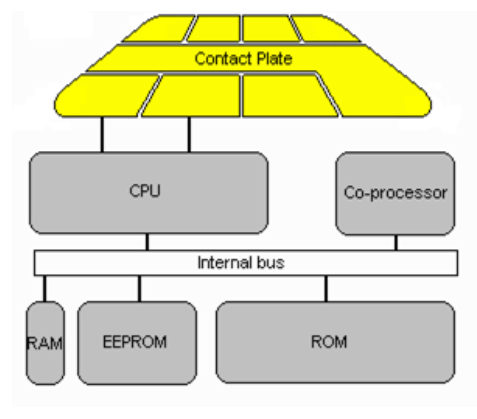
\includegraphics[width=0.6\linewidth]{Images/capitolo_2/smart_card_struttura.png}
\end{figure}

La tipica struttura hardware di una Smart Card è composta da:
\begin{itemize}
    \item \textbf{Contact plate}: i contatti metallici esterni utilizzati per effettuare le operazioni di I/O (Input/Output).
    \item \textbf{Processore (CPU)}: per eseguire le operazioni di calcolo e crittografia basilari.
    \item \textbf{ROM}: una piccola memoria a sola lettura che contiene il sistema operativo di base.
    \item \textbf{EEPROM}: funge da memoria semi-permanente, agendo di fatto come il disco fisso della carta. Nei vecchi telefoni cellulari, ad esempio, la rubrica e gli SMS venivano salvati esattamente qui.
    \item \textbf{RAM}: memoria volatile che ha la stessa identica funzione di quella presente in un classico computer.
\end{itemize}

Per quanto riguarda il Sistema Operativo, storicamente si trattava di software molto semplici e tendenzialmente monofunzione. Tuttavia, con la continua evoluzione di questi dispositivi, si è arrivati ad avere dei veri e propri OS nel senso moderno del termine. Grazie alle \textbf{Javacard}, ad esempio, è possibile eseguire bytecode direttamente sul chip. Un aneddoto molto interessante (nato dal celebre meme dell'informatica "\textit{Can it run Doom?}") è un progetto recente in cui una smart card è stata riprogrammata per rendere possibile l'esecuzione del gioco Doom (1993), dimostrando quanto questi "mini-computer" siano diventati potenti.

\section{Standard ISO 7816 e Attacchi}
Lo \textbf{Standard ISO 7816} è la normativa internazionale che definisce le proprietà fisiche e logiche richieste a una smart card. Tra i requisiti fisici previsti ci sono, ad esempio, l'immunità ai raggi UV e l'impenetrabilità del chip (che dovrebbe essere progettato per distruggersi piuttosto che lasciarsi ispezionare fisicamente).

La realtà dei fatti, però, è che la protezione fisica assoluta non può essere garantita. Nonostante gli standard, i malintenzionati riescono a mettere a punto attacchi veri e propri per aggirare le difese, riuscendo in alcuni casi a effettuare il dump dell'intera EEPROM, a clonare la carta o ad alterare i dati sensibili in essa contenuti.

\subsection{Tipologie di Attacco}
Possiamo dividere in generale gli attacchi alle smart card in due grandi macro-categorie:
\begin{itemize}
    \item \textbf{Invasivi}: richiedono di andare a manipolare fisicamente l'hardware della carta (es. rimuovendo strati del chip con acidi), finendo tendenzialmente per rovinare o distruggere l'involucro originale.
    \item \textbf{Non invasivi}: cercano di forzare o analizzare la carta (es. studiandone i consumi elettrici) senza agire fisicamente sulla sua struttura interna, preservandone così lo stato originale.
\end{itemize}
In generale, la tipica strategia di attacco è quella di effettuare attacchi invasivi in laboratorio per poi andare a effettuare attacchi non invasivi in serie.

\subsection*{Microprobing}
Il \textbf{Microprobing} è un classico attacco di tipo invasivo, estremamente complesso e costoso, che richiede attrezzatura di laboratorio specializzata. Generalmente si compone dei seguenti step:
\begin{itemize}
    \item \textbf{Depackaging}: estrazione fisica del chip di silicio dall'involucro di plastica della carta.
    \item \textbf{Riambientazione}: pulizia e preparazione del chip (spesso usando acidi per rimuovere gli strati protettivi superiori).
    \item \textbf{Ricostruzione del disegno (Reverse Engineering)}: analisi al microscopio per mappare i collegamenti e i bus interni.
    \item \textbf{Alterazioni manuali}: posizionamento di micro-sonde (probe) direttamente sui circuiti del chip.
    \item \textbf{Lettura della memoria}: intercettazione dei segnali elettrici per estrarre i dati.
\end{itemize}

Un attacco di questo genere è mirato a fare il \textit{dump} di informazioni sensibili che normalmente sarebbero inaccessibili. Ad esempio, la chiave a lungo termine salvata nella EEPROM, prima o poi, deve essere inviata alla CPU per eseguire le operazioni crittografiche. In quel preciso istante, la chiave viaggia in chiaro sui bus interni della carta e le micro-sonde possono intercettarla. 
Un principio simile (seppur non a livello di microprobing, ma di terminale) vale per la lettura del PIN: quando inseriamo il codice per un pagamento, questo passa in chiaro per un brevissimo tratto prima di essere cifrato. È in questa fase che agiscono i dispositivi malevoli (come gli \textit{skimmer}), motivo per cui è sempre sconsigliato l'inserimento della carta in macchinette o terminali non ufficiali o manomessi.

\subsection*{Attacchi Software}
Un classico esempio di attacco software non invasivo è quello storicamente perpetrato ai danni delle \textbf{Pay-TV}. Questi sistemi sfruttano una smart card per passare una chiave crittografica al decoder, il quale può così decodificare il segnale video. 
Nel momento in cui un cliente smette di pagare l'abbonamento, il gestore invia un messaggio di annullamento al decoder per disabilitare la smart card. L'attacco, in questo caso, non forza direttamente la crittografia della carta, ma consiste nel modificare il software del decoder affinché filtri o ignori del tutto questi messaggi di annullamento, permettendo alla smart card di continuare a decodificare il segnale a tempo indeterminato.

\subsection*{Eavesdropping (Side-Channel) e Fault Induction}
Queste tecniche si basano sull'osservazione e sulla manipolazione del comportamento fisico della carta durante il suo normale funzionamento:
\begin{itemize}
    \item \textbf{Eavesdropping (Analisi dei consumi)}: Monitorando minuziosamente il consumo di corrente sulle linee di alimentazione della smart card, un attaccante può riconoscere i pattern di assorbimento energetico. Poiché istruzioni diverse (es. moltiplicazione vs. addizione) consumano quantità di corrente diverse, è possibile risalire alla chiave crittografica utilizzata durante i calcoli.
    \item \textbf{Fault Induction (Iniezione di errori)}: In questo caso, l'attaccante va a indurre volontariamente un \textit{flip di bit} o un malfunzionamento (glitch) per ottenere effetti specifici. Ad esempio, inviando impulsi elettromagnetici precisi o abbassando repentinamente il voltaggio (glitch di corrente), si forza la carta a comportarsi in modo anomalo. I risultati vengono poi studiati tramite complessi esperimenti di analisi differenziale.
\end{itemize}

Un esempio storico e celebre di \textit{Fault Induction} è il glitch di corrente che esponeva la memoria dei microcontrollori \textbf{PIC16C84}. Di seguito possiamo vederne la logica vulnerabile:

\begin{figure}[H]
    \centering
    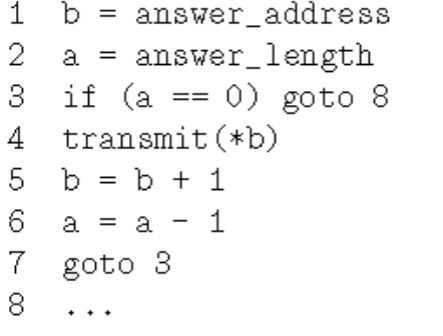
\includegraphics[width=0.6\linewidth]{Images/capitolo_2/glitch_corrente.png}
    \caption{Ciclo di trasmissione vulnerabile a glitch}
\end{figure}

Come possiamo intuire analizzando il codice, il chip utilizza una variabile \texttt{a} come contatore per la lunghezza del messaggio da trasmettere. Se un attaccante riesce a indurre un \textit{glitch} di corrente nel momento esatto in cui viene eseguita la riga 6 (\texttt{a = a - 1}) o il controllo alla riga 3 (\texttt{if (a == 0)}), la condizione di uscita dal ciclo fallisce. Di conseguenza, il ciclo continua all'infinito o va in underflow, facendo sì che il comando \texttt{transmit(*b)} alla riga 4 esegua il dump non solo della risposta prevista, ma dell'intera memoria del dispositivo.

